\section{Empirical illustration}
\label{sec:illustration}

The preceding sections describe the components of \pkg{amore} in isolation.
This section ties them together into the workflow a practitioner actually
runs, on two of the nine bundled datasets (Section~\ref{sec:software-data}): a
small, homogeneous face-to-face stream (\texttt{classroom\_events}) and a
larger, heavy-tailed email network (\texttt{radoslaw\_email}). The first
reproduces the central methodological lesson of \citet{juozaitiene2024} ---
that the count family silently absorbs actor heterogeneity --- and shows how
a sender frailty term diagnoses it. The second illustrates the smooth
backend recovering non-monotone effect shapes. All numbers and figures
restated below are produced by the package's reproducible driver
(\texttt{paper/wiki/experiments/realdata.R}) and are reported, unchanged,
from the package's real-data analysis article; we do not re-estimate them
here.

Before either fit, it is worth recalling why these two streams stress the
machinery differently. The bundled event-rate trace
(Figure~\ref{fig:illustration-rate}) shows that the datasets are emphatically
non-stationary: the classroom stream has two sharp spikes (its two recorded
sessions) on an otherwise quiet baseline, whereas the manufacturing email
stream carries a visible weekly modulation over a roughly stationary base
rate. The per-actor degree distributions differ even more sharply ---
\texttt{classroom\_events} is bell-shaped on a tight log axis (a small
homogeneous group), while \texttt{radoslaw\_email} is heavy-tailed across
orders of magnitude, a small core driving most of the traffic. That
heterogeneity is precisely what the count family can mistake for dynamics.

\begin{figure}[t]
  \centering
  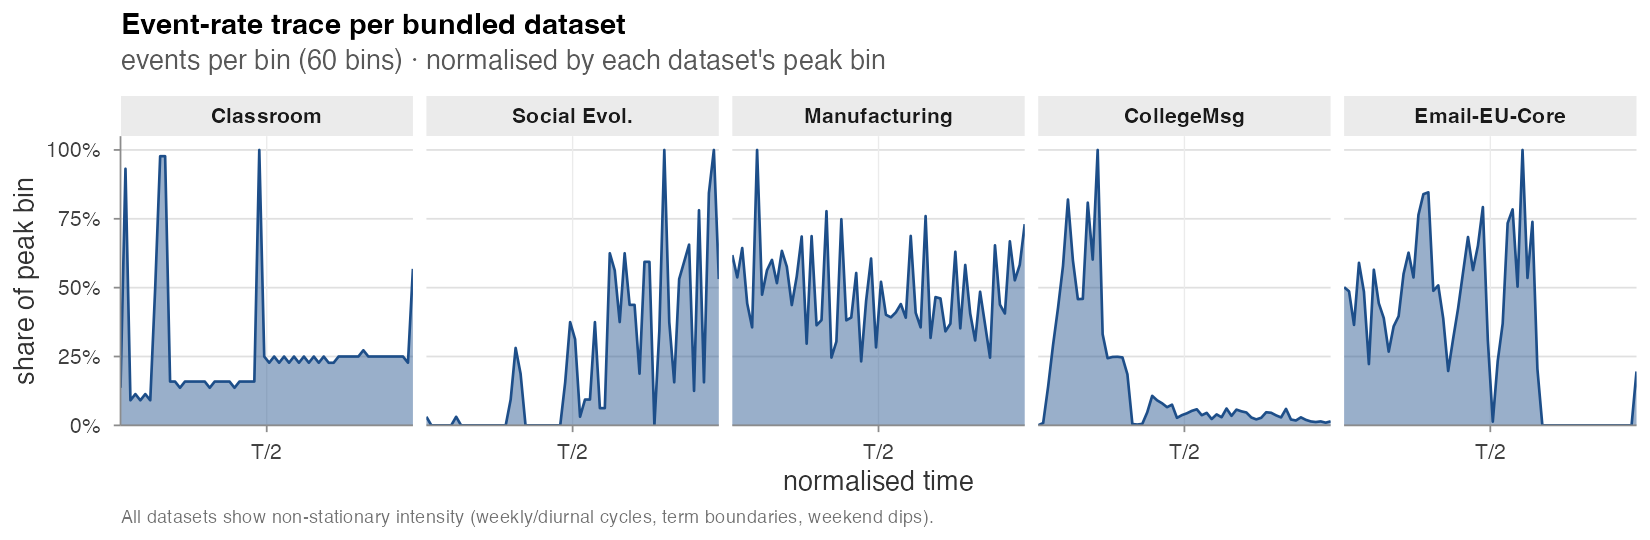
\includegraphics[width=0.95\textwidth]{figs/datasets-rate.png}
  \caption{Per-bin event-rate traces for the bundled datasets. The classroom
  stream (two session spikes) and the manufacturing email stream (weekly
  modulation on a stationary base) span the two regimes exercised in this
  section.}
  \label{fig:illustration-rate}
\end{figure}

\subsection{The common workflow}
\label{sec:illustration-workflow}

Every analysis in \pkg{amore} follows the same three steps: draw a
case--control sample of non-events, attach the endogenous statistics to the
resulting strata, and fit. The first two steps are backend-agnostic; only
the final \code{rem()} call (or, for the actor-heterogeneity diagnostic
below, \code{compare\_models()}) chooses an estimator. In code:

\begin{verbatim}
data(classroom_events)

cc   <- sample_non_events(classroom_events, n_controls = 3, seed = 11)
feat <- compute_endogenous_features(
  cc, stats = c("reciprocity_time_recent", "transitivity_time_recent"),
  history_log = classroom_events)

fit  <- rem(event ~ reciprocity_time_recent + transitivity_time_recent,
            data = feat, method = "clogit")
\end{verbatim}

\noindent The \code{sample\_non\_events()} call materialises, for each
observed event, a risk set of three sampled non-events; \code{compute\_%
endogenous\_features()} evaluates the requested statistics on the true
network history at each event time --- passing the original
stream as \code{history\_log} is essential here, so that only realised
events update the running network state while sampled controls read it
without writing to it (the alignment requirement established by experiment
E5 of Section~\ref{sec:validation}); and \code{rem(method =
"clogit")} maximises the risk-set softmax conditional-logistic partial
likelihood over the resulting strata. Swapping \code{method = "gam"}
substitutes the algebraically related degenerate case--control logistic
regression and unlocks \code{mgcv} smooth and time-varying terms;
\code{method = "nn"} substitutes the pure-R neural backend, which maximises
the same partial likelihood as \code{clogit} but scores the full candidate
vector jointly. The data frame \code{feat} is reused verbatim across all
three.

\subsection{Classroom: sender frailty flips the AIC ranking}
\label{sec:illustration-classroom}

The classroom stream (691 events, 20 actors, recorded in minutes;
\citealp{McFarland2001}) is small enough to refit repeatedly, which makes it
the natural vehicle for the actor-heterogeneity lesson. We compare three
effect specifications --- a \emph{count} family, a \emph{continuous}
(time-since-last) family, and the \emph{interrupted} variant of
\citet{juozaitiene2024} --- using \code{compare\_models()}, which wraps the
sample/feature/fit pipeline and returns an AIC table:

\begin{verbatim}
specs <- list(
  count       = c("reciprocity_count", "transitivity_count"),
  continuous  = c("reciprocity_time_recent", "transitivity_time_recent"),
  interrupted = c("reciprocity_time_recent_interrupted",
                  "transitivity_time_recent_interrupted"))

compare_models(classroom_events, specs, n_controls = 3, seed = 11)
#>         model n_terms n_obs  log_lik      AIC delta_AIC
#> 1       count       2   691 -5248.2 11880.5     0.0
#> 2  continuous       2   691 -5368.1 12120.2   239.7
#> 3 interrupted       2   691 -5449.8 12283.6   403.1
\end{verbatim}

Read naively, the count specification wins decisively, by 240 AIC points
over the continuous family. This is the trap: on a dataset with
heterogeneous senders the \texttt{*\_count} statistics absorb activity
differences directly, so they fit better for a reason that has nothing to do
with the timing dynamics the analyst cares about. The diagnostic is to add a
Gamma sender frailty (a \code{survival::frailty()} random effect on the
sender) and refit:

\begin{verbatim}
compare_models(classroom_events, specs, n_controls = 3, seed = 11,
               random_effects = "sender")
#>         model n_terms n_obs  log_lik      AIC delta_AIC
#> 1  continuous       2   691 -5177.7 11776.8     0.0
#> 2  interrupted       2   691 -5269.4 11960.5   183.7
#> 3       count       2   691      NA      NA     NA
\end{verbatim}

Two things happen, both shown in Figure~\ref{fig:realdata-classroom-flip}.
First, the count specification no longer fits at all: once the random effect
absorbs the activity differences, the inner Newton--Raphson update of the
frailty Cox fit fails to converge, and its AIC is undefined. Second, the
ranking among the remaining specifications flips --- continuous now overtakes
interrupted by 184 AIC points, matching Table~3 of \citet{juozaitiene2024}.
The lesson generalises: on heavy-tailed streams the naive AIC ranking
reflects who is active, not how the network evolves, and an actor-%
heterogeneity correction is the way to tell the two apart.

\begin{figure}[t]
  \centering
  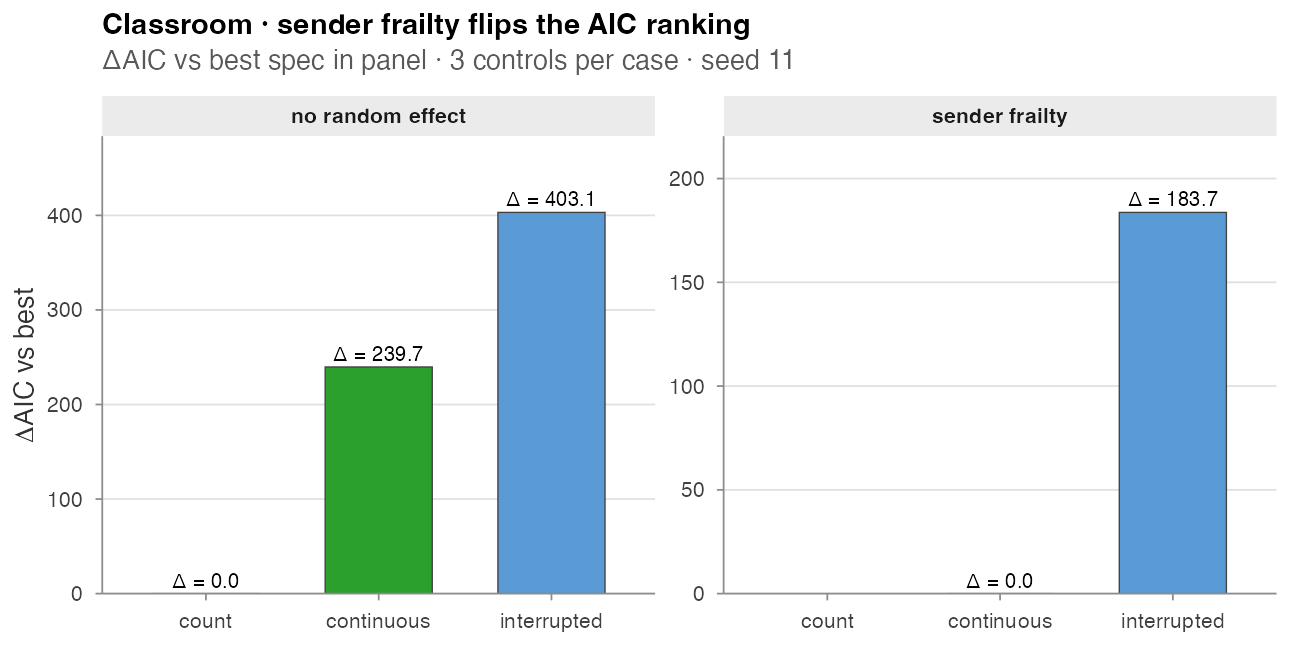
\includegraphics[width=0.9\textwidth]{figs/realdata-classroom-flip.png}
  \caption{Classroom AIC comparison without (left) and with (right) a Gamma
  sender frailty. Without the correction the count family leads by 240 AIC
  points; with it the count specification fails to converge and continuous
  overtakes interrupted by 184 points, reproducing Table~3 of
  \citet{juozaitiene2024}.}
  \label{fig:realdata-classroom-flip}
\end{figure}

\subsection{Manufacturing email: smooth effect curves}
\label{sec:illustration-smooth}

The same workflow, with \code{method = "gam"} in place of \code{clogit},
recovers the \emph{shape} of an endogenous effect rather than a single
coefficient. We use the first 30 days of the manufacturing email stream
(\texttt{radoslaw\_email}; \citealp{michalski2014}), restricted to
non-self-loops, and request smooth (penalised-spline) terms on four
statistics --- the continuous reciprocity and transitivity effects and their
interrupted variants:

\begin{verbatim}
data(radoslaw_email)
re30 <- radoslaw_email[radoslaw_email$time < 30, ]
re30 <- re30[re30$sender != re30$receiver, ]

stat_names <- c("reciprocity_time_recent",
                "transitivity_time_recent",
                "reciprocity_time_recent_interrupted",
                "transitivity_time_recent_interrupted")

cc   <- sample_non_events(re30, n_controls = 3, seed = 11)
feat <- compute_endogenous_features(cc, stats = stat_names)
\end{verbatim}

\noindent Fitting penalised splines on each statistic (via the smooth
backend, equivalently a stratified \code{pspline} Cox fit) yields the four
partial-effect curves in Figure~\ref{fig:realdata-manufacturing-smooth}. The
panels are not redundant. The continuous variants (top row) show the
canonical \emph{boost-then-decay} shape: a recent event briefly raises the
hazard, after which the contribution falls off and turns negative. The
interrupted variants (bottom row) start near zero, dip to a pronounced
minimum, and partially recover --- the cycle-closure-reset behaviour the
interrupted family is built to expose. Once the closing event fires, the
statistic snaps to a fresh state, and the partial effect on subsequent
events reflects that reset. A purely linear specification would collapse
each of these curves to a single slope and miss the non-monotonicity
entirely; this is the regime in which the smooth backend earns its place.

\begin{figure}[t]
  \centering
  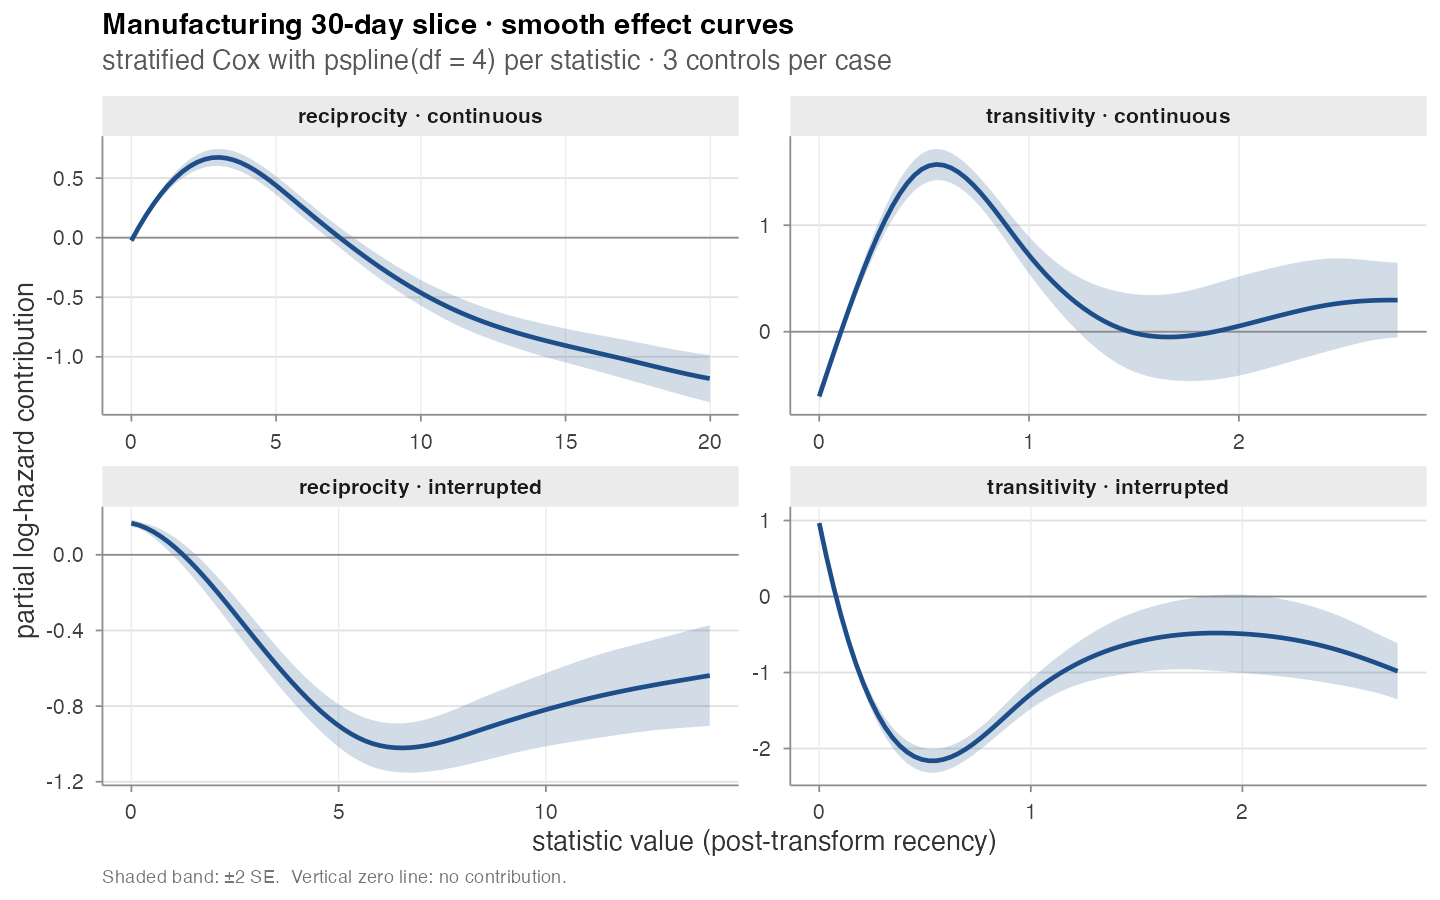
\includegraphics[width=0.95\textwidth]{figs/realdata-manufacturing-smooth.png}
  \caption{Penalised-spline partial-effect curves on the first 30 days of the
  manufacturing email stream. Continuous reciprocity and transitivity (top)
  show boost-then-decay; their interrupted variants (bottom) show the
  cycle-closure-reset dip and partial recovery.}
  \label{fig:realdata-manufacturing-smooth}
\end{figure}

\subsection{What the illustration does and does not show}
\label{sec:illustration-scope}

Taken together, the two analyses exercise the full front end on real data:
case--control sampling, the endogenous-statistics engine, the linear
conditional-logit fit, the smooth backend, and an actor-heterogeneity
diagnostic, all sharing one data structure. Two honest caveats apply. First,
the worked examples here use the \code{clogit} and \code{gam} backends; the
neural \code{nn} backend is demonstrated separately on a controlled planted-%
interaction design (Section~\ref{sec:validation}), where ground truth is
available, rather than on these streams, because its concordance figures are
in-sample and it carries no uncertainty quantification. Second, the
goodness-of-fit family (Section~\ref{sec:software-gof}) applies to the linear
case--control fit only; it is not exercised on the smooth manufacturing fit.
Within those bounds, the illustration demonstrates that the consolidated
workflow reproduces a published methodological finding
(\citealp{juozaitiene2024}, Table~3) end to end, from \code{data()} to AIC
table, in a single package.
